\documentclass[a4paper]{article}

% Global settings
\usepackage[utf8]{inputenc}
\usepackage[russian]{babel}
\usepackage[T1, T2A]{fontenc}

% For picture settings
\usepackage{graphicx}
\usepackage{float}
\usepackage{subfigure}
\usepackage{wrapfig}
\usepackage{caption}

% For typographic design
\usepackage[justification=centering]{caption}
\usepackage{geometry}
\usepackage{microtype}
\usepackage{indentfirst}
\usepackage{titling}
\usepackage{verbatim}
\usepackage{fancyhdr}
\usepackage{hyperref}
\usepackage{listings}
\usepackage{xcolor}
\usepackage{multirow}
\renewcommand{\refname}{Список литературы}

\definecolor{codegreen}{rgb}{0,0.6,0}
\definecolor{codegray}{rgb}{0.5,0.5,0.5}
\definecolor{codepurple}{rgb}{0.58,0,0.82}
\definecolor{backcolour}{rgb}{0.95,0.95,0.92}

\lstdefinestyle{coding}{
    backgroundcolor=\color{backcolour},   
    commentstyle=\color{codegreen},
    keywordstyle=\color{magenta},
    numberstyle=\tiny\color{codegray},
    stringstyle=\color{codepurple},
    basicstyle=\ttfamily\footnotesize,
    breakatwhitespace=false,         
    breaklines=true,                 
    captionpos=b,                    
    keepspaces=true,                 
    numbers=left,                    
    numbersep=5pt,                  
    showspaces=false,                
    showstringspaces=false,
    showtabs=false,                  
    tabsize=4
}

\pagestyle{fancy}
\fancypagestyle{titlingpage}{
    \fancyhead{}
    \renewcommand\headrulewidth{0pt}
    \fancyfoot[C]{\position , \the\year}
}
\fancypagestyle{main}{
    \fancyhead{}
    \renewcommand\headrulewidth{0pt}
    \fancyfoot[C]{\thepage}   
}

% For math support
\usepackage{enumerate}
\usepackage{amsmath}
\usepackage{amssymb}
\usepackage{cases}
\usepackage{bm}

% Settings
\linespread{2}
\geometry{scale=0.7}
\captionsetup{font = {scriptsize}}
\setlength\parindent{0pt}
\lstset{style=coding}

% Page Info
\title{«Автоматизированное тестирование»}
\author{Гуй Цици}
\newcommand{\authorinfo}{гр. 5130201/10101}
\newcommand{\director}{Курочкин Михаил Александрович}
\newcommand{\subject}{«Методы тестирования программного обеспечения»}
\newcommand{\tema}{Отчет по дисциплине}
\newcommand{\directortitle}{}
\newcommand{\otherpageinfo}{}
\newcommand{\position}{Санкт-Петербург}

% Begin document
\begin{document}

    % First page
    \makeatletter
    \begin{titlepage}
        \thispagestyle{titlingpage}
        \begin{center}
            \large{МИНОБРНАУКИ РОССИИ} \\

            \footnotesize{ФЕДЕРАЛЬНОЕ ГОСУДАРСТВЕННОЕ БЮДЖЕТНОE ОБРАЗОВАТЕЛЬНОЕ УЧРЕЖДЕНИЕ} \\
            \footnotesize{ВЫСШЕГО ПРОФЕССИОНАЛЬНОГО ОБРАЗОВАНИЯ} \\

            \textbf{«САНКТ-ПЕТЕРБУРГСКИЙ ПОЛИТЕХНИЧЕСКИЙ УНИВЕРСИТЕТ ПЕТРА ВЕЛИКОГО»} \\

            \normalsize{Институт компьютерных наук и кибербезопасности} \\
            \normalsize{Высшая школа технологий искусственного интеллекта} \\
            \normalsize{Направление 02.03.01 Математика и компьютерные науки} \\

            \hfill \break
            
            % For centralize
            \vspace*{\fill}
            \large{\tema} \\
            \subject \\
            \large{\textbf{\@title}} \\
            \textit{\otherpageinfo}

            \vspace*{\fill}

            \begin{tabular}{ccc}
                Студент: & \authorinfo & \@author \\
                Преподаватель: & \directortitle & \director
            \end{tabular}
            \hfill \break \hfill \break
        \end{center}
    \end{titlepage}

    \newpage
    \makeatother
    \thispagestyle{empty}
    \tableofcontents
    \newpage
    \pagestyle{main}
    \setlength{\parindent}{2em}

    \section*{Введение}
    \addcontentsline{toc}{section}{Введение}
    \noindent В лабораторных работах по автоматизированному тестированию требуется:
    \begin{itemize}
        \item С помощью фреймворка JUnit разработать unit-тесты к методам предоставленного класса Калькулятор. Необходимо протестировать 4 метода калькулятора;
        \item Используя фреймворк TestNG и методы библиотеки Selenium WebDriver реализовать 2 теста для предоставленного сайта в соответствии с заданием;
        \item Выполнить задания из второй лабораторной работы, используя шаблон проектирования тестов Page Object;
        \item Выполнить задания из третьей лабораторной работы с помощью шаблона Steps и, используя, Jenkins CI, создать задачу, которая будет запускать тесты из данной работы и тест, переделанный так, чтобы он не проходил. Также требуется создавать отчет о выполнении тестирования с помощью Allure Report.
    \end{itemize}
    \newpage

    \section{Описание автоматизации тестирования}
    \subsection{TestNG}
    \noindent TestNG – это фреймворк для тестирования Java-приложений. Особенности TestNG:
    \begin{itemize}
        \item Поддержка аннотаций;
        \item Поддержка тестирования интегрированных классов, например, по умолчанию нет необходимости создавать новый экземпляр класса теста для каждого метода тестирования;
        \item Разделение тестового кода времени компиляции и информации о конфигурации, данных времени выполнения.
        \item Гибкая конфигурация во время выполнения;
        \item Наличие «тестовых групп»;
        \item Поддержка зависимых методов тестирования, параллельного тестирования, нагрузочного тестирования и частичного отказа;
        \item Гибкий плагин API;
        \item Поддержка многопоточного тестирования.
    \end{itemize}
    \noindent Написание теста обычно состоит из трех этапов:
    \begin{enumerate}
        \item Реализация бизнес-логики теста и добавление аннотации TestNG в код;
        \item Добавление информации о тесте, например, имя класса, группы, в которой его необходимо запускать и т. д.);
        \item Запуск TestNG.
    \end{enumerate}
    \subsection{JUnit}
    JUnit — это фреймворк для языка программирования Java, предназначенный для автоматического тестирования программ. Его основное назначение — модульное тестирование. \par
    Основные отличия JUnit от TestNG:
    \begin{itemize}
        \item Аннотации Before и After для осуществления действий до и после тестирования, являются общими для методов и классов;
        \item Группировка происходит отдельной аннотацией Suite, а не через "pom.xml";
        \item Параметризация через аннотации ParametrizedTest и CsvSource.
    \end{itemize}
    \subsection{Selenium WebDriver}
    Selenium WebDriver — библиотека для управления браузерами, основной продукт комплекта Selenium. Представляет из себя семейство драйверов для разных браузеров (Firefox, Edge, Google Chrome/Chromium, Internet Explorer, Safari, Opera) и набор клиентских библиотек на разных языках программирования для работы с драйверами. WebDriver поддерживает работу с языками Java, .Net (C\#), Python, Ruby, JavaScript. \par
    WebDriver напрямую отправляет команды браузеру, используя его API и получает результаты тестирования, то есть используется способ взаимодействия с браузером, максимально близкий к действиям обычного пользователя. \par
    Для работы с Webdriver необходимо иметь 3 основных программных компонента:
    \begin{itemize}
        \item Браузер, работу которого пользователь хочет автоматизировать. Это реальный браузер определённой версии, установленный на определённой ОС и имеющий свои настройки;
        \item Для управления браузером необходим драйвербраузера. Драйвер является веб-сервером, который запускает браузер и отправляет ему команды, а также закрывает его;
        \item Тест, который содержит набор команд на определённом языке программирования для драйвера браузера.
    \end{itemize}
    Основными сущностями в Selenium WebDriver являются:
    \begin{enumerate}
        \item WebDriver – самая важная сущность, ответственная за управление браузером. Основной ход теста строится именно вокруг экземпляра этой сущности;
        \item WebElement – представляет собой абстракцию над веб-элементом, например, кнопкой,ссылкой, полем ввода и т.п. WebElement инкапсулирует методы для взаимодействия пользователя с элементами и получения их текущего статуса;
        \item By – абстракция над локатором веб-элемента. Этот класс инкапсулирует информацию о селекторе, например, CSS-селектор, а также сам локатор элемента, то есть всю информацию, необходимую для того, чтобы найти нужный элемент на странице.
    \end{enumerate}
    \subsection{Page Object}
    Page Object - один из наиболее полезных и используемых архитектурных решений в автоматизации. Данный шаблон проектирования помогает инкапсулировать работу с отдельными элементами страницы, что позволяет использовать одни и те же объекты страниц в различных тестах, и, следовательно, позволяет уменьшить количество кода и его поддержку. использовать в различных тестах. Например, если изменился дизайн одной из страниц, то возникает необходимость внести изменения только в соответствующий класс, описывающий эту страницу. \par
    Основные преимущества использование паттерна Page Object:
    \begin{itemize}
        \item Разделение кода тестов и кода описания страниц;
        \item Объединение всех действий по работе с веб-страницей в одном месте.
    \end{itemize} \par
    Паттерн Page Object в Selenium реализован с помощью библиотеки PageFactory и класса страницы. Page Object представляет собой отдельный класс, содержащий локаторы элементов, методы для работы с ними и конструктор принимающий в качестве параметра объект WebDriver. Методы класса Page Object могут возвращать объекты других Page Object классов.
    \subsection{Jenkins}
    Jenkins — программная система с открытым исходным кодом на Java, предназначенная для обеспечения процесса непрерывной интеграции программного обеспечения. \par
    Непрерывная интеграция (Continuous Integration, CI) – это процесс разработки программного обеспечения, смысл которого заключается в постоянном соединении рабочих копий в общую линию разработки, и выполнении постоянных автоматизированных сборок проекта для быстрого выявления возможных ошибок и решения интеграционных проблем. \par
    Jenkins позволяет автоматизировать часть процесса разработки программного обеспечения, в котором не обязательно участие человека, обеспечивая функции непрерывной интеграции. Может собирать проекты с использованием Apache Ant и Apache Maven, а также выполнять произвольные сценарии оболочки и пакетные файлы Windows. Сборка может быть запущена разными способами, например, по событию фиксации изменений в системе управления версиями, по расписанию, по запросу на определённый URL, после завершения другой сборки в очереди. Кроме того, возможности Jenkins могут быть расширены с помощью плагинов. \par
    Основные преимущества Jenkins:
    \begin{itemize}
        \item Режим работы сразу в двух и более средах;
        \item Повышенная надежность развертываемого программного обеспечения;
        \item Уменьшение ошибок, связанных с человеческим фактором;
        \item Уменьшение затрат на персонал;
        \item Упрощение рабочего процесса за счеттого,что не возникает необходимости нанимать дорогостоящую команду опытных специалистов, т.к. с Jenkins справится небольшая группа сотрудников без специальной квалификации.
    \end{itemize}
    \subsection{Allure Framework}
    Allure Framework – популярный инструмент построения отчётов автотестов, упрощающий их анализ. Это гибкий и легкий инструмент, который позволяет получить не только краткую информацию о ходе выполнения тестов, но и предоставляет всем участникам производственного процесса максимум полезной информации из повседневного выполнения автоматизированных тестов. \par
    Разработчикам и тестировщикам использование отчетов Allure позволяет сократить жизненный цикл дефекта: падения тестов могут быть разделены на дефекты продукта и дефекты самого теста, что сокращает затраты времени на анализ дефекта и его устранение. Также к отчету могут быть прикреплены логи, обозначены тестовые шаги, добавлены вложения с разнообразным контентом, получена информация о таймингах и времени выполнения тестов. \par
    Кроме того, Allure-отчеты поддерживают взаимодействие с системами непрерывной интеграции и баг-трекинговыми системами, что позволяет всегда держать под рукой нужную информацию о прохождении тестов и дефектах. \par
    Тест-менеджерам Allure дает общее представление о работоспособности проекта, позволяет понять, какая часть проекта покрыта тестами, как сгруппированы дефекты, какова общая динамока качества проекта.

    \section{Результаты выполнения лабораторных работ}
    \subsection{Лабораторная работа №1}
    В данной работе было необходимо разработать unit-тесты к предоставленной библиотеке calculator-1.0.jar, которая содержит класс Калькулятор с методами, соответствующими операциям калькулятора. Было необходимо протестировать 4 операции. Тесты должны быть написаны с использованием фреймворка JUnit. \par
    В результате выполнения лабораторной работы было реализовано 8 классов: AddLongTest, AddDoubleTest, DivLongTest, DivDoubleTest, MulLongTest, MulDoubleTest, SubLongTest, SubDoubleTest. Всего было реализовано 96 тестов.
    \begin{lstlisting}[language=Java]
class AddDoubleTest extends AbstractCalculatorTest {
    @ParameterizedTest
    @ValueSource(doubles = { 0.0, -1.0, 1.0, 12345.67, -12345.67 })
    void testAdditionWithZero(double input) {
        assertEquals(input, calculator.sum(input, 0.0), DELTA);
    }

    @ParameterizedTest
    @ValueSource(doubles = { -1.0, 1.0, 12345.67, -12345.67 })
    void testAdditionWithSelf(double input) {
        assertEquals(input * 2, calculator.sum(input, input), DELTA);
    }

    @ParameterizedTest
    @CsvSource({ "5.7, 2.3, 3.4", "-2.5, -1.2, -1.3", "0.0, -5.5, 5.5" })
    void testGeneralCorrectness(double expected, double a, double b) {
        assertEquals(expected, calculator.sum(a, b), DELTA);
    }
}
class AddLongTest extends AbstractCalculatorTest {
    @ParameterizedTest
    @ValueSource(longs = { 0, -1, 1, 12345, -12345 })
    void testAdditionWithZero(long input) {
        assertEquals(input, calculator.sum(input, 0));
    }

    @ParameterizedTest
    @ValueSource(longs = { 0, -1, 1, 12345, -12345 })
    void testAdditionWithSelf(long input) {
        assertEquals(input * 2, calculator.sum(input, input));
    }

    @ParameterizedTest
    @CsvSource({ "5, 2, 3", "-2, -1, -1", "0, -5, 5" })
    void testGeneralCorrectness(long expected, long a, long b) {
        assertEquals(expected, calculator.sum(a, b));
    }
}
class DivDoubleTest extends AbstractCalculatorTest {
    @ParameterizedTest
    @ValueSource(doubles = { 0.0, -1.0, 1.0, 12345.67, -12345.67 })
    void testDivisionByZero(double input) {
        assertThrows(NumberFormatException.class, () -> calculator.div(input, 0.0));
    }

    @ParameterizedTest
    @ValueSource(doubles = { -1.0, 1.0, 12345.67, -12345.67 })
    void testDivisionByOne(double input) {
        assertEquals(input, calculator.div(input, 1.0), DELTA);
    }

    @ParameterizedTest
    @CsvSource({ "4.0, 20.0, 5.0", "-6.0, 36.0, -6.0", "-9.0, -72.0, 8.0" })
    void testGeneralCorrectness(double expected, double a, double b) {
        assertEquals(expected, calculator.div(a, b), DELTA);
    }
}
class DivLongTest extends AbstractCalculatorTest {
    @ParameterizedTest
    @ValueSource(longs = { 0, -1, 1, 12345, -12345 })
    void testDivisionByZero(long input) {
        assertThrows(NumberFormatException.class, () -> calculator.div(input, 0));
    }

    @ParameterizedTest
    @ValueSource(longs = { 0, -1, 1, 12345, -12345 })
    void testDivisionByOne(long input) {
        assertEquals(input, calculator.div(input, 1));
    }

    @ParameterizedTest
    @CsvSource({ "4, 20, 5", "-6, 36, -6", "-9, -72, 8" })
    void testGeneralCorrectness(long expected, long a, long b) {
        assertEquals(expected, calculator.div(a, b));
    }
}
class MulDoubleTest extends AbstractCalculatorTest {
    @ParameterizedTest
    @ValueSource(doubles = { 0.0, -1.0, 1.0, 12345.67, -12345.67 })
    void testMultiplicationWithZero(double input) {
        assertEquals(0.0, calculator.mult(input, 0.0), DELTA);
    }

    @ParameterizedTest
    @ValueSource(doubles = { -1.0, 1.0, 12345.67, -12345.67 })
    void testMultiplicationWithOne(double input) {
        assertEquals(input, calculator.mult(input, 1.0), DELTA);
    }

    @ParameterizedTest
    @CsvSource({ "6.0, 2.0, 3.0", "1.0, -1.0, -1.0", "0.0, -5.5, 0.0" })
    void testGeneralCorrectness(double expected, double a, double b) {
        assertEquals(expected, calculator.mult(a, b), DELTA);
    }
}
class MulLongTest extends AbstractCalculatorTest {
    @ParameterizedTest
    @ValueSource(longs = { 0, -1, 1, 12345, -12345 })
    void testMultiplicationWithZero(long input) {
        assertEquals(0, calculator.mult(input, 0));
    }

    @ParameterizedTest
    @ValueSource(longs = { -1, 1, 12345, -12345 })
    void testMultiplicationWithOne(long input) {
        assertEquals(input, calculator.mult(input, 1));
    }

    @ParameterizedTest
    @CsvSource({ "6, 2, 3", "1, -1, -1", "0, -5, 0" })
    void testGeneralCorrectness(long expected, long a, long b) {
        assertEquals(expected, calculator.mult(a, b));
    }
}
class SubDoubleTest extends AbstractCalculatorTest {
    @ParameterizedTest
    @ValueSource(doubles = { 0.0, -1.0, 1.0, 12345.67, -12345.67 })
    void testSubtractionWithZero(double input) {
        assertEquals(input, calculator.sub(input, 0.0), DELTA);
    }

    @ParameterizedTest
    @ValueSource(doubles = { -1.0, 1.0, 12345.67, -12345.67 })
    void testSubtractionWithSelf(double input) {
        assertEquals(0.0, calculator.sub(input, input), DELTA);
    }

    @ParameterizedTest
    @CsvSource({ "1.1, 3.2, 2.1", "0.0, -1.1, -1.1", "-10.5, -5.5, 5.0" })
    void testGeneralCorrectness(double expected, double a, double b) {
        assertEquals(expected, calculator.sub(a, b), DELTA);
    }
}
class SubLongTest extends AbstractCalculatorTest {
    @ParameterizedTest
    @ValueSource(longs = { 0, -1, 1, 12345, -12345 })
    void testSubtractionWithZero(long input) {
        assertEquals(input, calculator.sub(input, 0));
    }

    @ParameterizedTest
    @ValueSource(longs = { 0, -1, 1, 12345, -12345 })
    void testSubtractionWithSelf(long input) {
        assertEquals(0, calculator.sub(input, input));
    }

    @ParameterizedTest
    @CsvSource({ "1, 3, 2", "0, -1, -1", "-10, -5, 5" })
    void testGeneralCorrectness(long expected, long a, long b) {
        assertEquals(expected, calculator.sub(a, b));
    }
}\end{lstlisting}
    Результаты тестов представлены:
    \begin{figure}[H]
        \centering
        \begin{minipage}[t]{0.5\textwidth}
            \includegraphics[width=\textwidth]{images/lab1-test-result.png}
        \end{minipage}
        \caption{Результаты тестирования}
    \end{figure}
    \subsection{Лабораторная работа №2}
    В данной лабораторной работе необходимо использовать фреймворк TestNG для того, чтобы протестировать корректность работы библиотеки SeleniumWebDriver на примере сайта \url{https://jdi-testing.github.io/jdi-light/index.html} с использованием браузера Chrome. Необходимо реализовать два теста, каждый из которых проверяет корректность отображения конкретной страницы этого сайта. Ниже приведены представленные для работы тестовые сценарии.
    \begin{figure}[H]
        \centering
        \begin{minipage}[t]{0.7\textwidth}
            \includegraphics[width=\textwidth]{images/lab2-task1.png}
        \end{minipage}
        \caption{Тестовый сценарий 1}
    \end{figure}
    \begin{figure}[H]
        \centering
        \begin{minipage}[t]{0.7\textwidth}
            \includegraphics[width=\textwidth]{images/lab2-task2.png}
        \end{minipage}
        \caption{Тестовый сценарий 2}
    \end{figure} \par
    В результате выполнения были реализованы три класса: DriverSerup, SubTaskA и SubTaskB. Для запуска этих классов был создан Maven профиль.
    \begin{lstlisting}[language=Java]
public class DriverSetup {
    protected static WebDriver driver;

    @BeforeClass
    public void setup() {
        System.setProperty("webdriver.chrome.driver", "src/test/resources/chromedriver");
        System.setProperty("webdriver.http.factory", "jdk-http-client");
        driver = new ChromeDriver();
        driver.manage().window().maximize();

        // 1. Open test site by URL
        driver.navigate().to("https://jdi-testing.github.io/jdi-light/index.html");

        // 3. Perform login
        driver.findElement(
                By.cssSelector("html>body>header>div>nav>ul.uui-navigation.navbar-nav.navbar-right>li>a>span")).click();
        driver.findElement(By.id("name")).sendKeys("Roman");
        driver.findElement(By.id("password")).sendKeys("Jdi1234");
        driver.findElement(By.id("login-button")).click();
    }

    @AfterClass
    public void exit() {
        // 10. Close Browser
        driver.close();
    }
}
public class SubTaskA extends DriverSetup {
    @Test
    public void testTask() {
        SoftAssert softAssert = new SoftAssert();

        // 2. Assert browser title
        softAssert.assertEquals(driver.getTitle(), "Home Page");

        // 4. Assert Username is logged in
        softAssert.assertEquals(driver.findElement(By.id("user-name")).getText(), "ROMAN IOVLEV");

        // 5. Assert that there are 4 items on the header section are displayed, and they have proper texts
        List<WebElement> headerItems = driver.findElement(By.cssSelector("ul.uui-navigation.nav.navbar-nav.m-l8"))
                .findElements(By.xpath("./child::*"));
        final int EXPECTED_HEADER_ITEMS_SIZE = 4;
        softAssert.assertEquals(headerItems.size(), EXPECTED_HEADER_ITEMS_SIZE);
        headerItems.forEach(item -> softAssert.assertTrue(item.isDisplayed()));
        softAssert.assertEquals(headerItems.stream().map(WebElement::getText).toList(),
                List.of("HOME", "CONTACT FORM", "SERVICE", "METALS & COLORS"));

        // 6. Assert that there are 4 images on the Index Page, and they are displayed
        List<WebElement> benefitImages = driver.findElements(By.className("benefit-icon"));
        final int EXPECTED_BENEFIT_IMAGES_SIZE = 4;
        softAssert.assertEquals(benefitImages.size(), EXPECTED_BENEFIT_IMAGES_SIZE);
        benefitImages.forEach(image -> softAssert.assertTrue(image.isDisplayed()));

        // 7. Assert that there are 4 texts on the Index Page under icons, and they have proper text
        List<WebElement> benefitTexts = driver.findElements(By.className("benefit-txt"));
        final int EXPECTED_BENEFIT_TEXTS_SIZE = 4;
        softAssert.assertEquals(benefitTexts.size(), EXPECTED_BENEFIT_TEXTS_SIZE);
        benefitTexts.forEach(text -> softAssert.assertTrue(text.isDisplayed()));
        softAssert.assertEquals(
                benefitTexts.stream()
                        .map(WebElement::getText)
                        .map(text -> text.replace("\n", " "))
                        .toList(),
                List.of(
                        "To include good practices and ideas from successful EPAM project",
                        "To be flexible and customizable",
                        "To be multiplatform",
                        "Already have good base (about 20 internal and some external projects), wish to get more..."));

        // 8. Assert that there is the iframe with Frame Button exist
        final String EXPECTED_IFRAME_SRC = "https://jdi-testing.github.io/jdi-light/frame-button.html";
        softAssert.assertEquals(driver.findElement(By.tagName("iframe")).getAttribute("src"),
                EXPECTED_IFRAME_SRC);

        // 9.  Switch to the iframe and check that there is Frame Button in the iframe
        driver.switchTo().frame("frame");
        final String EXPECTED_FRAME_VALUE = "Frame Button";
        softAssert.assertEquals(driver.findElement(By.id("frame-button")).getAttribute("value"),
                EXPECTED_FRAME_VALUE);

        // 10. Switch to original window back
        driver.switchTo().defaultContent();

        // 11. Assert that there are 5 items in the Left Section are displayed, and they have proper text
        List<WebElement> leftSectionItems = driver.findElement(By.cssSelector("ul.sidebar-menu.left"))
                .findElements(By.xpath("./child::*"));
        leftSectionItems.forEach(item -> softAssert.assertTrue(item.isDisplayed()));
        softAssert.assertEquals(leftSectionItems.stream().map(WebElement::getText).toList(), List.of(
                "Home", "Contact form", "Service", "Metals & Colors", "Elements packs"));

        // Assert all in soft assert
        softAssert.assertAll();
    }
}
public class SubTaskB extends DriverSetup {
    @Test
    public void testBrowserTitle() {
        // 2. Assert browser title
        assertEquals(driver.getTitle(), "Home Page");
    }

    @Test
    public void testLogin() {
        // 4. Assert User name in the left-top side of screen that user is loggined
        assertEquals(driver.findElement(By.id("user-name")).getText(), "ROMAN IOVLEV");
    }

    @Test
    public void testElements() {
        // 5. Open through the header menu Service -> Different Elements Page
        driver.findElement(By.cssSelector("body>header>div>nav>ul.uui-navigation.nav.navbar-nav.m-l8>li>a>span"))
                .click();
        driver.findElement(By.xpath("html/body/header/div/nav/ul[1]/li[3]/ul/li[8]/a")).click();

        // 6. Select checkboxes
        driver.findElements(By.className("label-checkbox")).stream()
                .filter(checkbox -> checkbox.getText().equals("Water") || checkbox.getText().equals("Wind"))
                .forEach(WebElement::click);

        // 7. Select radio
        driver.findElements(By.className("label-radio")).stream()
                .filter(radio -> radio.getText().equals("Selen"))
                .forEach(WebElement::click);

        // 8. Select in dropdown
        driver.findElements(By.tagName("option")).stream()
                .filter(option -> option.getText().equals("Yellow"))
                .forEach(WebElement::click);

        // 9. Assert logs
        final int LOGS_BEGIN_INDEX = 9;
        List<String> logLines = Arrays.stream(driver.findElement(By.cssSelector("ul.panel-body-list.logs")).getText()
                .split("\n")).map(line -> line.substring(LOGS_BEGIN_INDEX))
                .toList();
        assertEquals(logLines, List.of(
                "Colors: value changed to Yellow",
                "metal: value changed to Selen",
                "Wind: condition changed to true",
                "Water: condition changed to true"));
    }
}\end{lstlisting}
    Результаты тестов:
    \begin{figure}[H]
        \centering
        \begin{minipage}[t]{0.6\textwidth}
            \includegraphics[width=\textwidth]{images/lab2-test-result.png}
        \end{minipage}
        \caption{Результаты тестирования сайта}
    \end{figure}
    \subsection{Лабораторная работа №3}
    В данной работе необходимо произвести рефакторинг тестов из второй лабораторной работы, используя шаблон проектирования тестов Page Object. То есть нужно создать объекты страниц и отделить код работы с элементами страницы от работы с веб-драйвером. \par
    В результате выполнения работы были реализованы классы HomePage, DifferentElementsPage, IFrame, представляющие 3 различных веб-страницы, и классы Header и LeftSection, представляющие 2 веб-элемента страницы HomePage, которые используются в процессе тестирования. После реализации необходимых средств для работы с вебстраницами был изменен код классов, содержащих тесты.
    \begin{lstlisting}[language=Java]
public class DifferentElementsPage {
    private static final Integer LOGS_BEGIN_INDEX = 9;

    @FindBy(className = "label-checkbox")
    private List<WebElement> checkboxes;

    @FindBy(className = "label-radio")
    private List<WebElement> radios;

    @FindBy(tagName = "option")
    private List<WebElement> dropdownOptions;

    @FindBy(css = "ul.panel-body-list.logs")
    private WebElement logs;

    public DifferentElementsPage(WebDriver webDriver, HomePage homePage) {
        homePage.getHeaderSection().clickServiceDropdown();
        homePage.getHeaderSection().clickDifferentElements();
        PageFactory.initElements(webDriver, this);
    }

    public void selectCheckbox(String name) {
        this.checkboxes.stream().filter(checkbox -> checkbox.getText().equals(name))
                .forEach(WebElement::click);
    }

    public void selectRadio(String name) {
        this.radios.stream().filter(radio -> radio.getText().equals(name))
                .forEach(WebElement::click);
    }

    public void selectDropdownOption(String name) {
        this.dropdownOptions.stream().filter(option -> option.getText().equals(name))
                .forEach(WebElement::click);
    }

    public List<String> getLogs() {
        return Arrays.stream(logs.getText().split("\n"))
                .map(log -> log.substring(LOGS_BEGIN_INDEX)).toList();
    }
}
public class DriverSetup {
    protected static WebDriver webDriver;
    protected static HomePage homePage;

    @BeforeClass
    public static void setup() {
        System.setProperty("webdriver.chrome.driver", "src/test/resources/chromedriver");
        System.setProperty("webdriver.http.factory", "jdk-http-client");
        Properties properties = new Properties();
        try {
            properties.load(Files.newInputStream(Path.of("src/test/resources/data.properties")));
        } catch (IOException error) {
            throw new RuntimeException(error);
        }

        webDriver = new ChromeDriver();
        webDriver.manage().window().maximize();

        homePage = new HomePage(webDriver, properties.getProperty("site.url"));

        // 3. Perform login
        homePage.performLogin(
                properties.getProperty("user.name"),
                properties.getProperty("user.password"));
    }

    @AfterClass
    public static void exit() {
        // 10. Close browser
        webDriver.close();
    }
}
public class ExpectedData {
    public static final String SITE_NAME = "Home Page";
    public static final String LOGGED_USER_NAME = "ROMAN IOVLEV";
    public static final List<String> HEADER_SECTION_ITEMS = List.of(
        "HOME", "CONTACT FORM", "SERVICE", "METALS & COLORS"
    );
    public static final List<String> BENEFIT_ICONS = List.of(
        "To include good practices\nand ideas from successful\nEPAM project",
        "To be flexible and\ncustomizable",
        "To be multiplatform",
        "Already have good base\n(about 20 internal and\nsome external projects),\nwish to get more..."
    );
    public static final List<String> LEFT_SECTION_ITEMS = List.of(
        "Home", "Contact form", "Service", "Metals & Colors", "Elements packs"
    );
    public static final List<String> DIFFERENT_ELEMENTS_LOGS = List.of(
        "Colors: value changed to Yellow",
        "metal: value changed to Selen",
        "Wind: condition changed to true",
        "Water: condition changed to true"
    );
}
public class HeaderSection {
    @FindBy(css = "body > header > div > nav > ul.uui-navigation.nav.navbar-nav.m-l8 > li")
    private List<WebElement> items;

    @FindBy(css = "body > header > div > nav > ul.uui-navigation.nav.navbar-nav.m-l8 > li > a > span")
    private WebElement serviceDropdown;

    @FindBy(css = "body > header > div > nav > ul.uui-navigation.nav.navbar-nav.m-l8 > li.dropdown.open > ul > li:nth-child(8) > a")
    private WebElement differentElements;

    public HeaderSection(WebDriver webDriver) {
        PageFactory.initElements(webDriver, this);
    }

    public void clickServiceDropdown() {
        this.serviceDropdown.click();
    }

    public void clickDifferentElements() {
        this.differentElements.click();
    }

    public List<WebElement> getItems() {
        return this.items;
    }

    public Integer getItemsSize() {
        return this.items.size();
    }

    public List<String> getItemsNames() {
        return this.items.stream().map(WebElement::getText).toList();
    }
}
public class HomePage {
    private final WebDriver webDriver;
    private final HeaderSection headerSection;
    private final LeftSection leftSection;

    @FindBy(id = "name")
    private WebElement loginUsername;

    @FindBy(id = "password")
    private WebElement loginPassword;

    @FindBy(css = "html > body > header > div > nav > ul.uui-navigation.navbar-nav.navbar-right > li > a > span")
    private WebElement loginDropdownButton;

    @FindBy(id = "login-button")
    private WebElement loginButton;

    @FindBy(id = "user-name")
    private WebElement username;

    @FindBy(className = "benefit-icon")
    private List<WebElement> benefitIcons;

    @FindBy(className = "benefit-txt")
    private List<WebElement> benefitIconsTexts;

    @FindBy(tagName = "iframe")
    private WebElement iframe;

    public HomePage(WebDriver webDriver, String url) {
        this.webDriver = webDriver;

        // 1. Open test site by URL
        this.webDriver.navigate().to(url);

        PageFactory.initElements(this.webDriver, this);
        headerSection = new HeaderSection(webDriver);
        leftSection = new LeftSection(webDriver);
    }

    public void performLogin(String username, String password) {
        this.loginDropdownButton.click();
        this.loginUsername.sendKeys(username);
        this.loginPassword.sendKeys(password);
        this.loginButton.click();
    }

    public String getTitle() {
        return this.webDriver.getTitle();
    }

    public String getLoggedName() {
        return this.username.getText();
    }

    public HeaderSection getHeaderSection() {
        return this.headerSection;
    }

    public Integer getBenefitIconsSize() {
        return this.benefitIcons.size();
    }

    public List<WebElement> getBenefitIcons() {
        return this.benefitIcons;
    }

    public Integer getBenefitIconsTextsSize() {
        return this.benefitIconsTexts.size();
    }

    public List<String> getBenefitIconsTextsStrings() {
        return this.benefitIconsTexts.stream().map(WebElement::getText).toList();
    }

    public LeftSection getLeftSection() {
        return this.leftSection;
    }

    public WebElement getFrame() {
        return this.iframe;
    }

    public WebElement getFrameButton() {
        return new IFrame(this.webDriver).getFrameButton();
    }

    public void switchToOriginalWindow() {
        this.webDriver.switchTo().defaultContent();
    }
}
public class IFrame {
    @FindBy(id = "frame-button")
    private WebElement frameButton;

    public IFrame(WebDriver webDriver) {
        webDriver.switchTo().frame("frame");
        PageFactory.initElements(webDriver, this);
    }

    public WebElement getFrameButton() {
        return this.frameButton;
    }
}
public class LeftSection {
    @FindBy(css = "#mCSB_1_container > ul > li")
    private List<WebElement> items;

    public LeftSection(WebDriver webDriver) {
        PageFactory.initElements(webDriver, this);
    }

    public List<WebElement> getItems() {
        return this.items;
    }

    public Integer getItemSize() {
        return this.items.size();
    }

    public List<String> getItemsNames() {
        return this.items.stream().map(WebElement::getText).toList();
    }
}
public class SubTaskA extends DriverSetup {
    @Test
    public void testTaskA() {
        SoftAssert softAssert = new SoftAssert();

        // 2. Assert browser title
        softAssert.assertEquals(homePage.getTitle(), ExpectedData.SITE_NAME);

        // 4. Assert user is logged in
        softAssert.assertEquals(homePage.getLoggedName(), ExpectedData.LOGGED_USER_NAME);

        // 5. Assert that there are 4 items on the header section are displayed , and they have proper texts
        softAssert.assertEquals((int) homePage.getHeaderSection().getItemsSize(), (int) ExpectedData.HEADER_SECTION_ITEMS.size());
        softAssert.assertEquals(homePage.getHeaderSection().getItemsNames(), ExpectedData.HEADER_SECTION_ITEMS);
        homePage.getHeaderSection().getItems().forEach(item -> {
            softAssert.assertTrue(item.isDisplayed());
        });

        // 6. Assert that there are 4 images on the Index Page, and they are displayed
        softAssert.assertEquals((int) homePage.getBenefitIconsSize(), (int) ExpectedData.BENEFIT_ICONS.size());
        homePage.getBenefitIcons().forEach(icon -> {
            softAssert.assertTrue(icon.isDisplayed());
        });

        // 7. Assert that there are 4 texts on the Index Page under icons, and they have proper text
        softAssert.assertEquals((int) homePage.getBenefitIconsTextsSize(), (int) ExpectedData.BENEFIT_ICONS.size());
        softAssert.assertEquals(homePage.getBenefitIconsTextsStrings(), ExpectedData.BENEFIT_ICONS);

        // 8. Assert that there is an iframe with frame button exists
        softAssert.assertTrue(homePage.getFrame().isDisplayed());

        // 9. Switch to the iframe and check that there is Frame Button in the iframe
        softAssert.assertTrue(homePage.getFrameButton().isDisplayed());

        // 10. Switch to original window back
        homePage.switchToOriginalWindow();

        // 11. Assert that there are 5 items in the Left Section are displayed, and they have proper text
        softAssert.assertEquals((int) homePage.getLeftSection().getItemSize(), (int) ExpectedData.LEFT_SECTION_ITEMS.size());
        homePage.getLeftSection().getItems().forEach(item -> {
            softAssert.assertTrue(item.isDisplayed());
        });
        softAssert.assertEquals(homePage.getLeftSection().getItemsNames(), ExpectedData.LEFT_SECTION_ITEMS);

        softAssert.assertAll();
    }
}
public class SubTaskB extends DriverSetup {
    @Test
    public void testBrowserTitle() {
        // 2. Assert browser title
        assertEquals(homePage.getTitle(), ExpectedData.SITE_NAME);
    }

    @Test
    public void testLogin() {
        // 4. Assert user is logged in
        assertEquals(homePage.getLoggedName(), ExpectedData.LOGGED_USER_NAME);
    }

    @Test
    public void testElements() {
        // 5. Open through the header menu Service -> Different Elements Page
        DifferentElementsPage differentElementsPage = new DifferentElementsPage(webDriver, homePage);

        // 6. Select checkboxes
        differentElementsPage.selectCheckbox("Water");
        differentElementsPage.selectCheckbox("Wind");

        // 7. Select radio
        differentElementsPage.selectRadio("Selen");

        // 8. Select in dropdown
        differentElementsPage.selectDropdownOption("Yellow");

        // 9. Assert logs
        assertEquals(differentElementsPage.getLogs(), ExpectedData.DIFFERENT_ELEMENTS_LOGS);
    }
}\end{lstlisting}
    Результаты тестов:
    \begin{figure}[H]
        \centering
        \begin{minipage}[t]{0.6\textwidth}
            \includegraphics[width=\textwidth]{images/lab3-test-result.png}
        \end{minipage}
        \caption{Результаты тестирования сайта}
    \end{figure}
    \subsection{Лабораторная работа №4}
    В данной лабораторной работе необходимо произвести рефакторинг тестов из лабораторной работы 3 с использованием шаблона программирования Steps. То есть необходимо создать еще один уровень между кодом тестов и кодом взаимодействия с веб-страницами и веб-элементами. Классы с шагами будут отвечать за вызов определенных методов для действий на странице и за запуск проверок. Таким образом, код теста будет состоять из вызовов реализованных шагов. \par
    Кроме того, необходимо создать третий тест на основе теста из предыдущей работы, который бы содержал ошибки и оказался не пройденным. \par
    Также необходимо создать задачу в Jenkins, которая будет запускать полученные тесты и создавать отчет с помощью Allure Report.
    \begin{lstlisting}[language=Java]
public class Action extends StepsSetup {
    public Action(WebDriver webDriver, Properties properties) {
        super(webDriver, properties);
    }

    @Step("Navigating to Home Page")
    public void navigateToHomePage() {
        homePage = new HomePage(webDriver, properties.getProperty("site.url"));
    }

    @Step("Logging in")
    public void performLogin() {
        homePage.performLogin(
                properties.getProperty("user.name"),
                properties.getProperty("user.password"));
    }

    @Step("Switching to the original window")
    public void switchToOriginalWindow() {
        homePage.switchToOriginalWindow();
    }

    @Step("Navigating to different elements page")
    public void navigateToDifferentElementsPage() {
        differentElementsPage = new DifferentElementsPage(webDriver, homePage);
    }

    @Step("Selecting checkboxes")
    public void selectCheckboxes(String... names) {
        Stream.of(names).forEach(name -> differentElementsPage.selectCheckbox(name));
    }

    @Step("Selecting radio")
    public void selectRadio(String name) {
        differentElementsPage.selectRadio(name);
    }

    @Step("Selecting dropdown option")
    public void selectDropdownOption(String name) {
        differentElementsPage.selectDropdownOption(name);
    }
}
public class Assertion extends StepsSetup {
    public Assertion(WebDriver webDriver, Properties properties) {
        super(webDriver, properties);
    }

    @Step("Asserting Home Page's title")
    public void assertHomePageTitle(String expectedTitle) {
        assertEquals(homePage.getTitle(), expectedTitle);
    }

    @Step("Asserting user is logged in")
    public void assertUserLoggedIn(String expectedUsername) {
        assertEquals(homePage.getLoggedName(), expectedUsername);
    }

    @Step("Asserting Header Seciton items properties")
    public void assertHeaderSectionItemsProperties(
            Integer expectedItemsSize,
            List<String> expectedItemsNames) {
        SoftAssert softAssert = new SoftAssert();
        softAssert.assertEquals(homePage.getHeaderSection().getItemsSize(), expectedItemsSize);
        softAssert.assertEquals(homePage.getHeaderSection().getItemsNames(), expectedItemsNames);
        homePage.getHeaderSection().getItems().forEach(item -> {
            softAssert.assertTrue(item.isDisplayed());
        });
        softAssert.assertAll();
    }

    @Step("Asserting Index Page images properties")
    public void assertIndexPageImages(Integer expectedImagesSize) {
        SoftAssert softAssert = new SoftAssert();
        softAssert.assertEquals(homePage.getBenefitIconsSize(), expectedImagesSize);
        homePage.getBenefitIcons().forEach(icon -> {
            softAssert.assertTrue(icon.isDisplayed());
        });
        softAssert.assertAll();
    }

    @Step("Asserting Index Page texts properties")
    public void assertIndexPageTexts(
            Integer expectedTextsSize,
            List<String> expectedTextsStrings) {
        SoftAssert softAssert = new SoftAssert();
        softAssert.assertEquals(homePage.getBenefitIconsTextsSize(), expectedTextsSize);
        softAssert.assertEquals(homePage.getBenefitIconsTextsStrings(), expectedTextsStrings);
        softAssert.assertAll();
    }

    @Step("Asserting iframe existence")
    public void assertFrameExsitence() {
        assertTrue(homePage.getFrame().isDisplayed());
    }

    @Step("Asserting Frame Button existence")
    public void assertFrameButtonExistence() {
        assertTrue(homePage.getFrameButton().isDisplayed());
    }

    @Step("Asserting Left Section properties")
    public void assertLeftSectionProperties(
            Integer expectedItemsSize,
            List<String> expectedItemsNames) {
        SoftAssert softAssert = new SoftAssert();
        softAssert.assertEquals(homePage.getLeftSection().getItemSize(), expectedItemsSize);
        softAssert.assertEquals(homePage.getLeftSection().getItemsNames(), expectedItemsNames);
        homePage.getLeftSection().getItems().forEach(item -> {
            softAssert.assertTrue(item.isDisplayed());
        });
        softAssert.assertAll();
    }

    @Step("Asserting logs")
    public void assertLogs(List<String> logs) {
        assertEquals(differentElementsPage.getLogs(), logs);
    }
}
@Feature("First task using Steps")
public class SubTaskA extends DriverSetup {
    @Story("Testing the Home Page")
    @Test
    public void testTaskA() {
        // 2. Assert browser title
        assertion.assertHomePageTitle(ExpectedData.SITE_NAME);

        // 4. Assert user is logged in
        assertion.assertUserLoggedIn(ExpectedData.LOGGED_USER_NAME);

        // 5. Assert that there are 4 items on the header section are displayed, and they have proper texts
        assertion.assertHeaderSectionItemsProperties(
                ExpectedData.HEADER_SECTION_ITEMS.size(),
                ExpectedData.HEADER_SECTION_ITEMS);

        // 6. Assert that there are 4 images on the Index Page, and they are displayed
        assertion.assertIndexPageImages(ExpectedData.BENEFIT_ICONS.size());

        // 7. Assert that there are 4 texts on the Index Page under icons, and they have proper text
        assertion.assertIndexPageTexts(ExpectedData.BENEFIT_ICONS.size(), ExpectedData.BENEFIT_ICONS);

        // 8. Assert that there is the iframe with frame button exists
        assertion.assertFrameExsitence();

        // 9. Switch to the iframe and check that there is Frame Button in the iframe
        assertion.assertFrameButtonExistence();

        // 10. Switch to original window back
        action.switchToOriginalWindow();

        // 11. Assert that there are 5 items in the Left Section are displayed, and they have proper text
        assertion.assertLeftSectionProperties(
                ExpectedData.LEFT_SECTION_ITEMS.size(),
                ExpectedData.LEFT_SECTION_ITEMS);
    }
}
@Feature("Second task using Steps")
public class SubTaskB extends DriverSetup {
    @Story("Testing the Different Elements page")
    @Test
    public void testTaskB() {
        // 2. Assert browser title
        assertion.assertHomePageTitle(ExpectedData.SITE_NAME);

        // 4. Assert user is logged in
        assertion.assertUserLoggedIn(ExpectedData.LOGGED_USER_NAME);

        // 5. Open through the header header menu Service -> Different Elements Page
        action.navigateToDifferentElementsPage();

        // 6. Select checkboxes
        action.selectCheckboxes("Water", "Wind");

        // 7. Select radio
        action.selectRadio("Selen");

        // 8. Select item in dropdown
        action.selectDropdownOption("Yellow");

        // 9. Assert logs
        assertion.assertLogs(ExpectedData.DIFFERENT_ELEMENTS_LOGS);
    }
}
public class BadTask extends DriverSetup {
    @Test
    public void testBadTask() {
        // 2. Assert browser title - a random stirng :)
        assertion.assertHomePageTitle("A WRONG SITENAME");
    }
}\end{lstlisting}
    Результаты тестов:
    \begin{figure}[H]
        \centering
        \begin{minipage}[t]{\textwidth}
            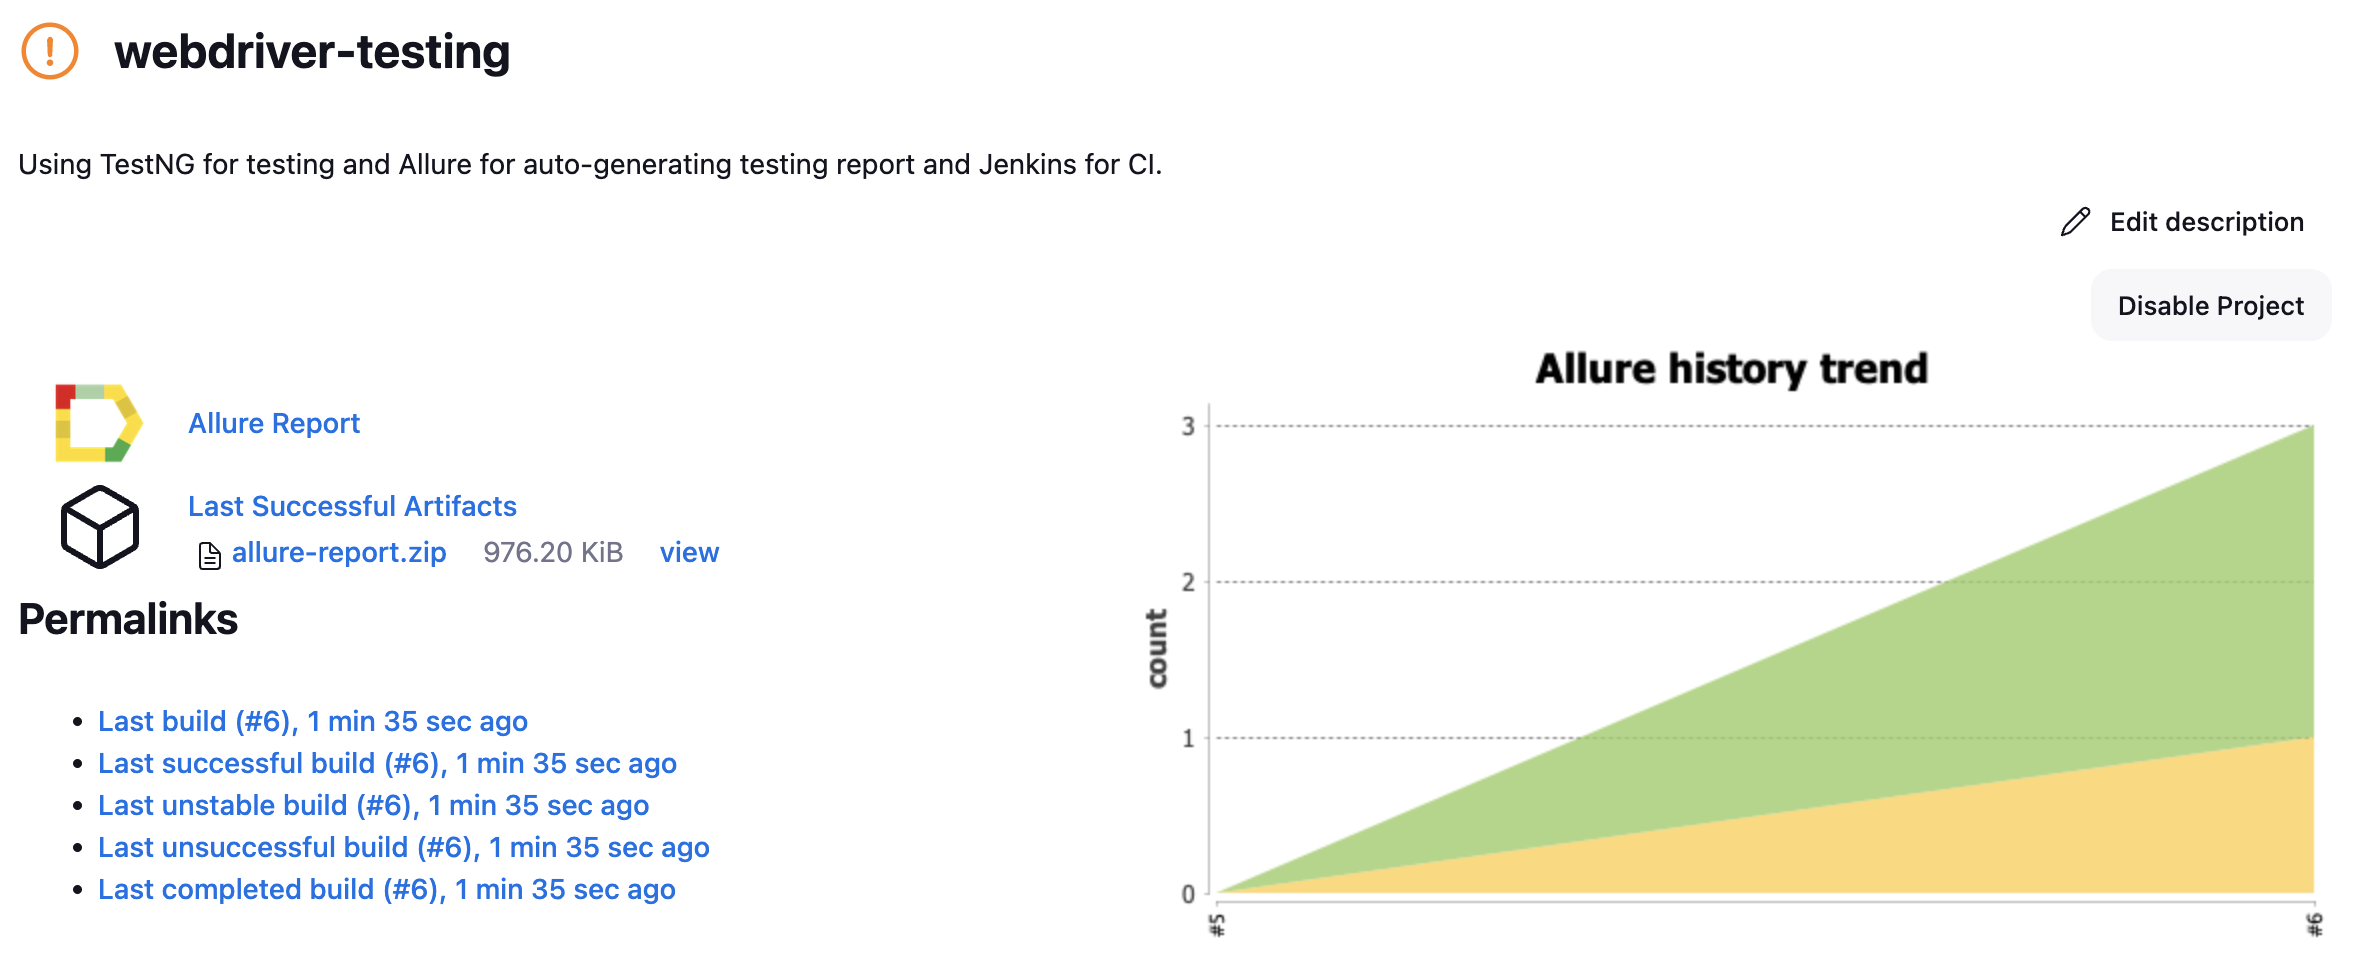
\includegraphics[width=\textwidth]{images/jenkins-allure-result.png}
        \end{minipage}
        \caption{Задача в Jenkins}
    \end{figure}
    \begin{figure}[H]
        \centering
        \begin{minipage}[t]{\textwidth}
            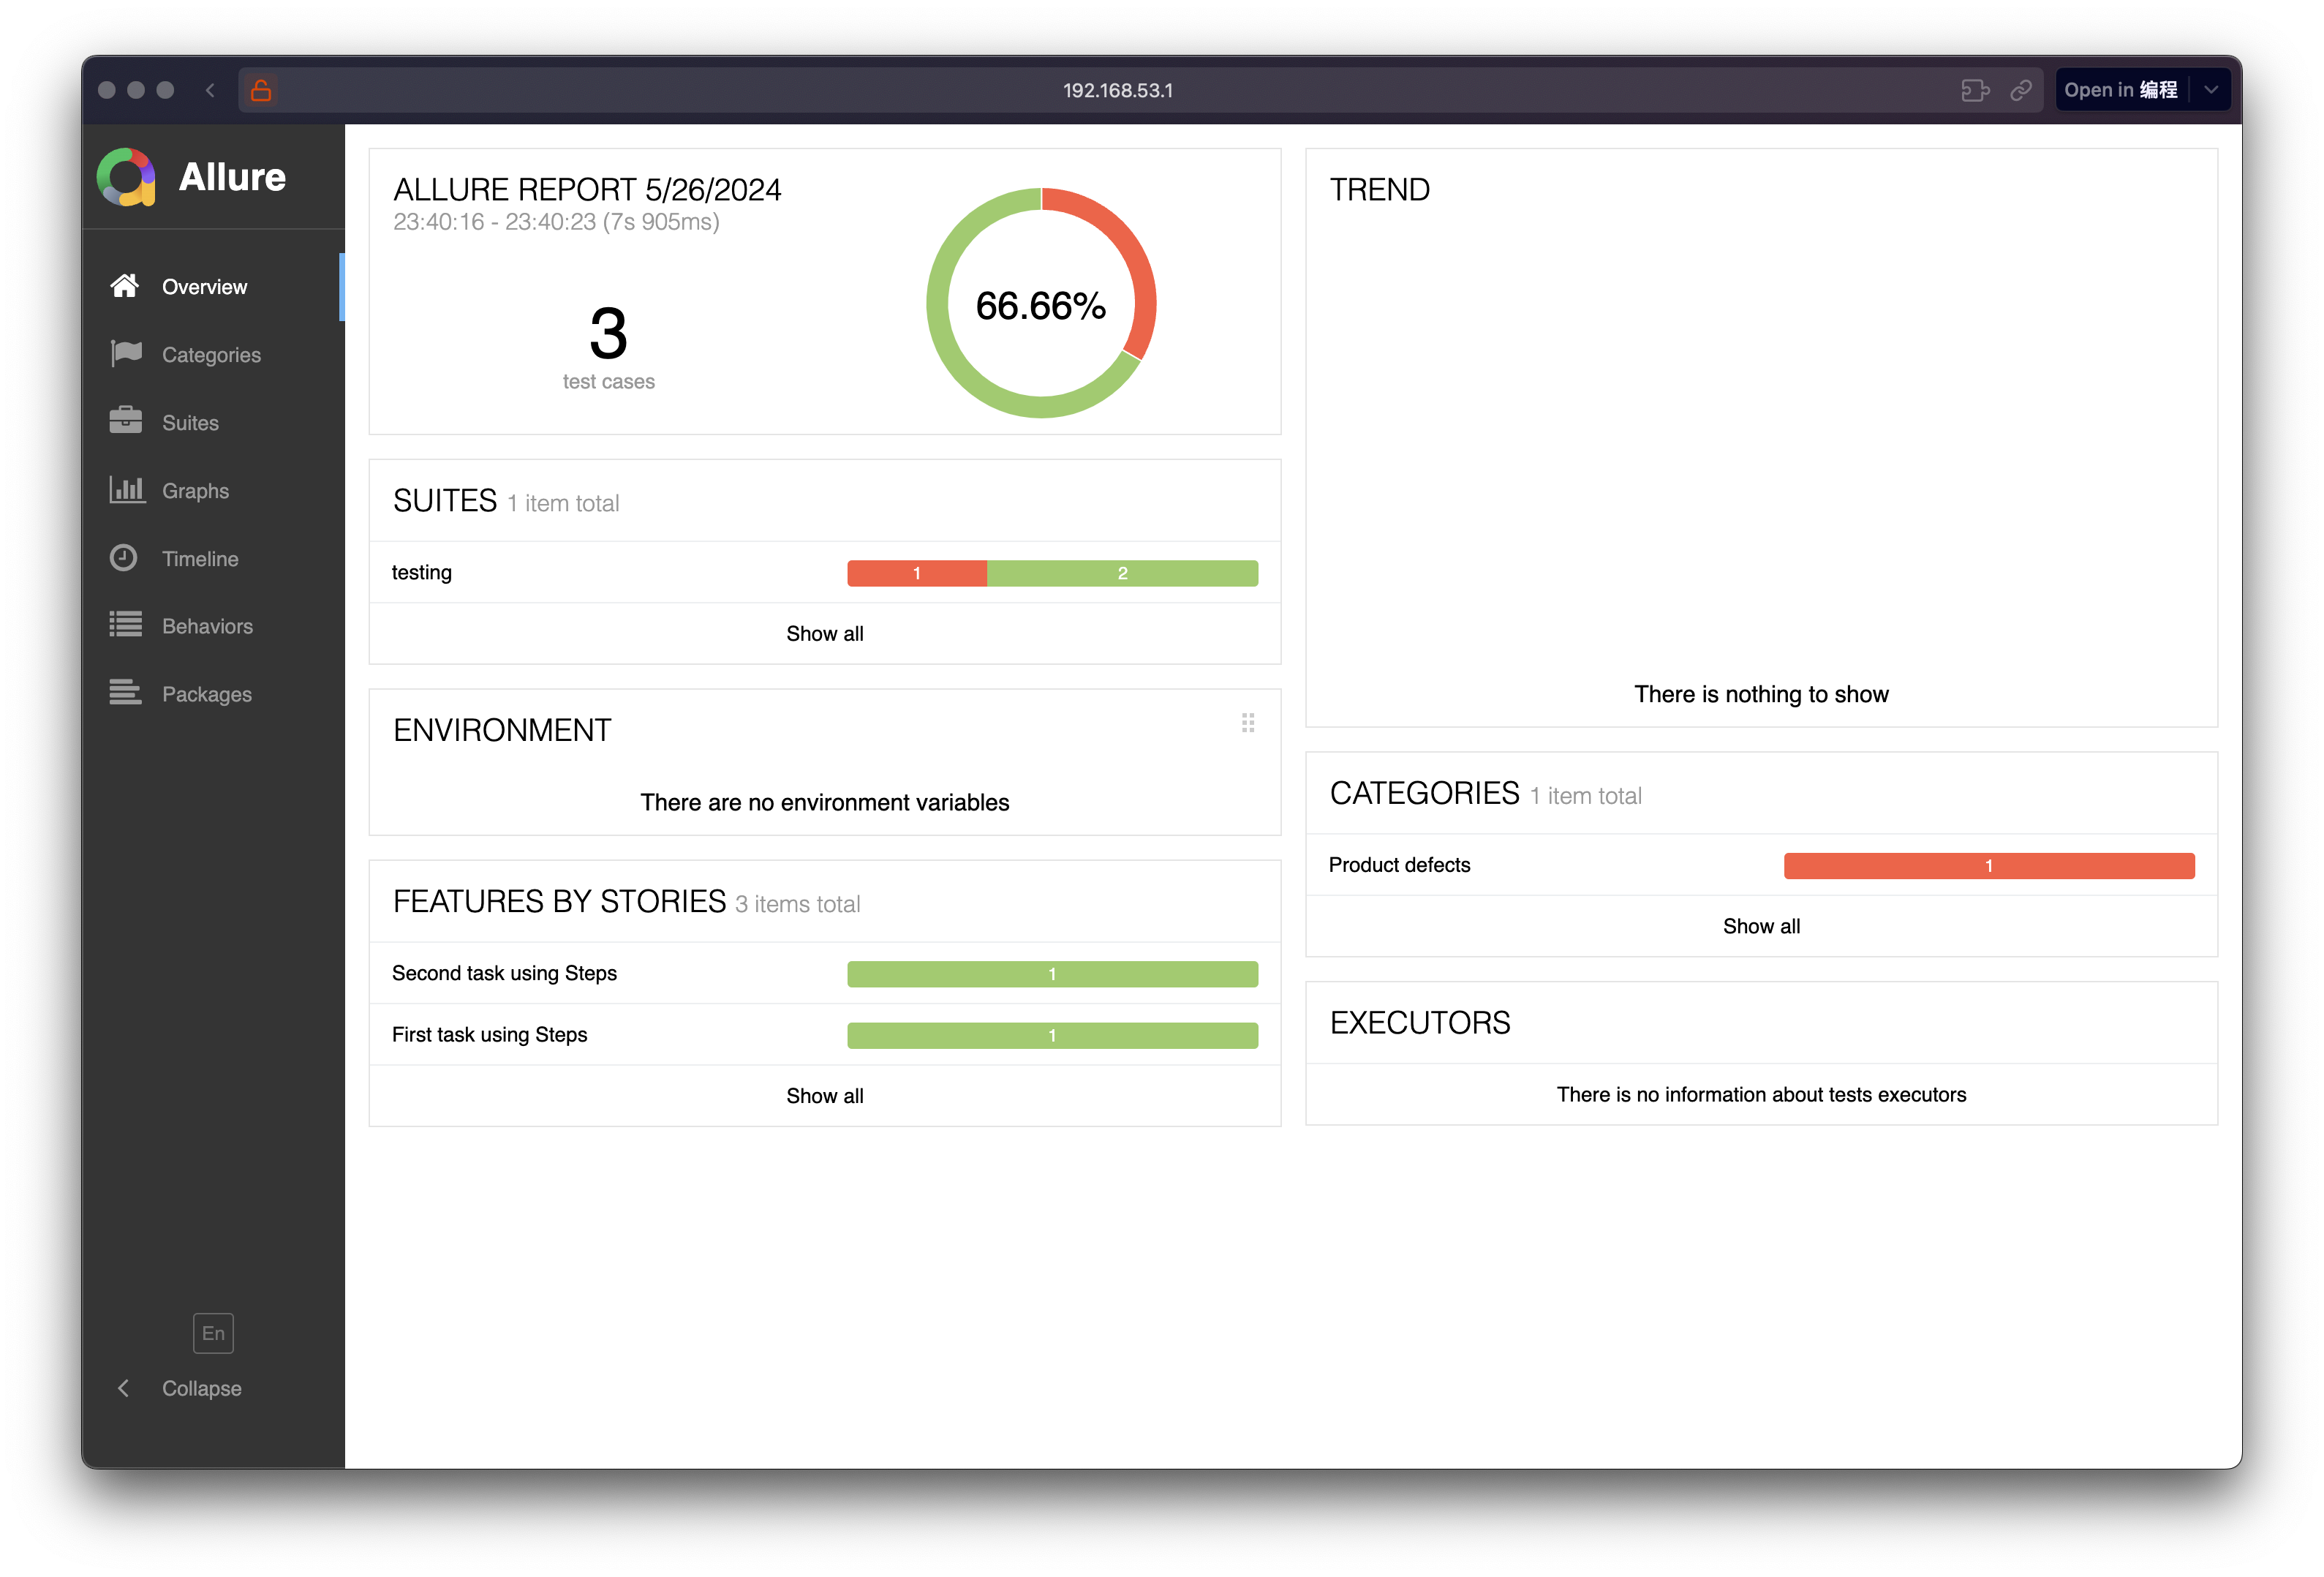
\includegraphics[width=\textwidth]{images/allure-result.png}
        \end{minipage}
        \caption{Сформированный отчет в Allure}
    \end{figure}
    \newpage

    \section*{Заключение}
    \addcontentsline{toc}{section}{Заключение}
    В результате прохождения курса были изучены такие инструменты для автоматизации тестирования ПО, как фреймворки JUnit, TestNG, библиотека для управления браузерами Selenium WebDriver, шаблоны проектирования автоматизированных тестов Page Object и Steps, программная система сборки проектов Jenkins, фреймворк для создания отчетов Allure Framework. \par
    Полученные знания были применены на практике в процессе выполнения 4 лабораторных работ. Все работы были выполнены успешно. \par
    Тестирование, выполняемое с помощью специализированного ПО, позволяет ускорить процесс тестирования, не понижая при этом его качество, устранить влияние человеческого фактора, а также достаточно быстро и легко получить наглядные результаты тестирования с помощью составления отчетов. Используемые при автоматизированном тестировании шаблоны проектирования позволяют формализовать структуру кода тестов.
    \newpage

    \begin{thebibliography}{2}
        \bibitem{textbook}
        Майерс, Г. Искусство тестирования программ / Г. Майерс, Т. Баджетт, К. Сандлер. Изд. 3-е. — Санкт-Петербург : Диалектика, 2012. — 272 c.
        \bibitem{course}
        Курс лекций по атоматизированному тестированию. Башарина Е.А. Шукшин И.Д.
    \end{thebibliography}
    \newpage
    
\end{document}